\documentclass{beamer}
% \usepackage{enumitem}
\usepackage{float}
\usetheme{Boadilla}
\usepackage{graphicx} % Required for inserting images

\title{Image Segmentation with PCUNet}
\author{Deeksha Dhiwakar, Shravan Srinivasa Raghavan}

\begin{document}

\maketitle
\begin{frame}{Introduction}
    
Image segmentation plays a vital role in healthcare for extracting key information from complex images of tissues and organs .
Our focus is on a specific paper in this field, which provides an innovative method for extracting information from
ovarian tissues. The paper chosen is Orian Tumor Ultrasound Image Segmentation
with Deep Neural Networks.
\end{frame}
\begin{frame}{Existing Technology in the Field}
    The U-Net already exist and has demonstrated remarkable success in the field of medical image computing. However due to its
    small receptive field, U-Net faces challenges in extracting global context information. This paper presents a U-Net based
    network named PCU-Net for segmentation of ovarian tumors incorporating ConvMixer and Pyramid Dilated Convolution (PDC modules)

\end{frame}

\begin{frame}{The UNet }
\begin{figure}[H]
        \centering
        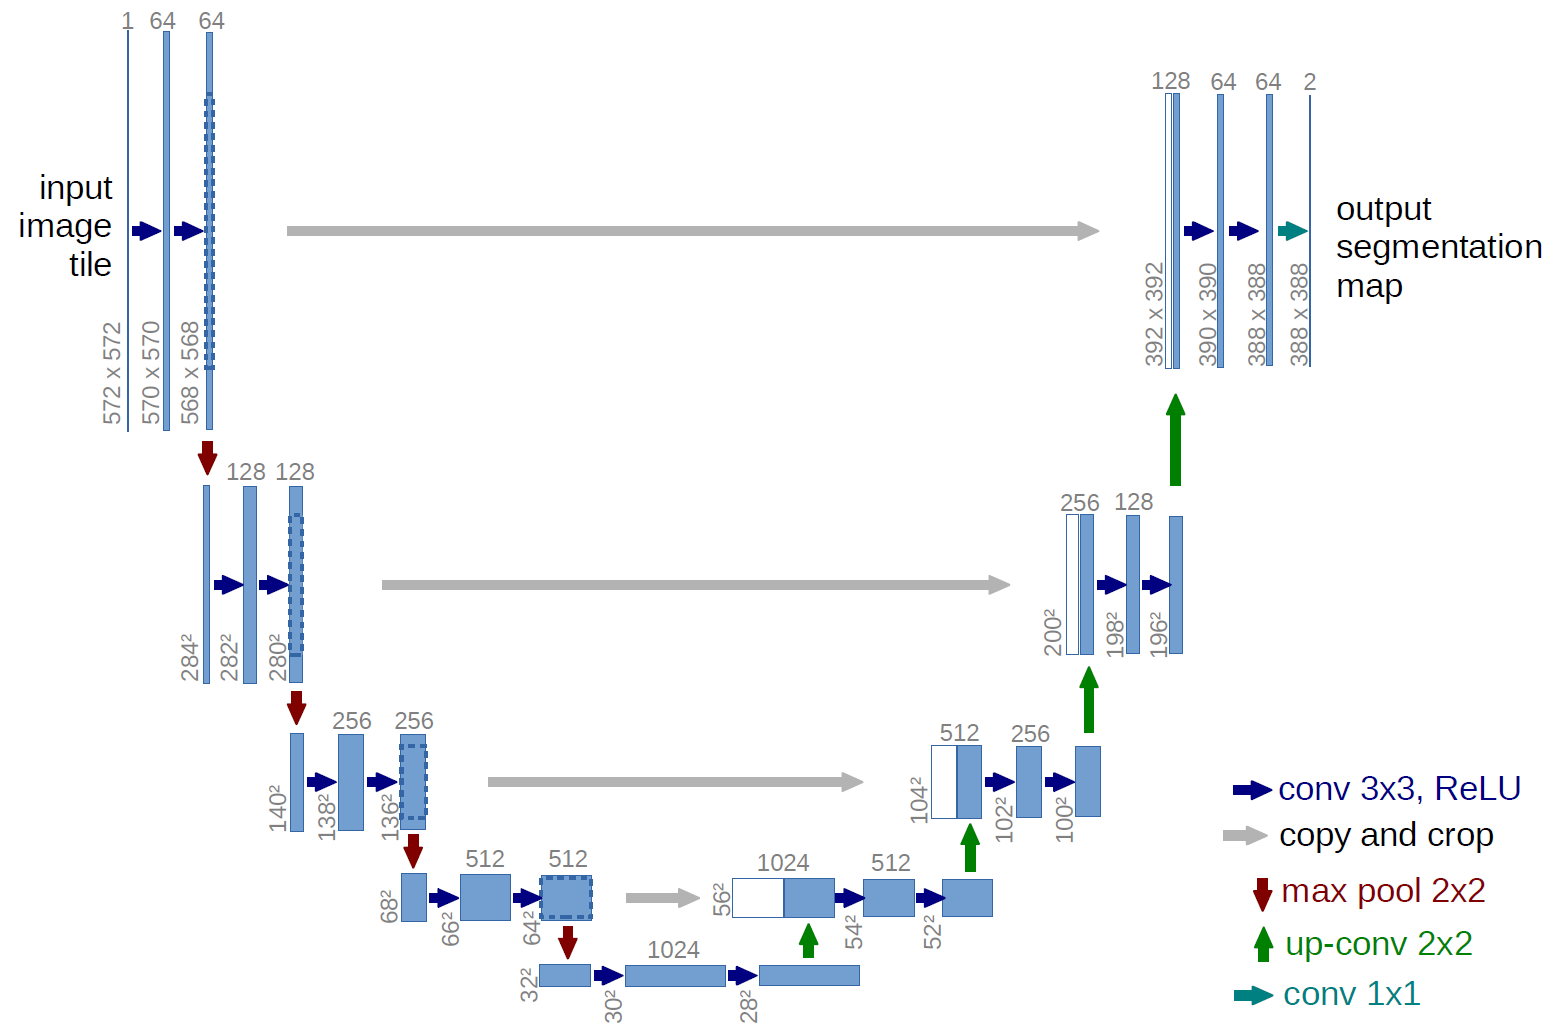
\includegraphics[width=0.6\textwidth]{u-net-architecture.png}
        \caption{The U-Net}
        \label{fig:a}
\end{figure}

\end{frame}
\begin{frame}{The Conv Mixer and PDC Layer}
    \begin{figure}[H]
    \begin{minipage}[b]{0.5\linewidth}
        \centering
        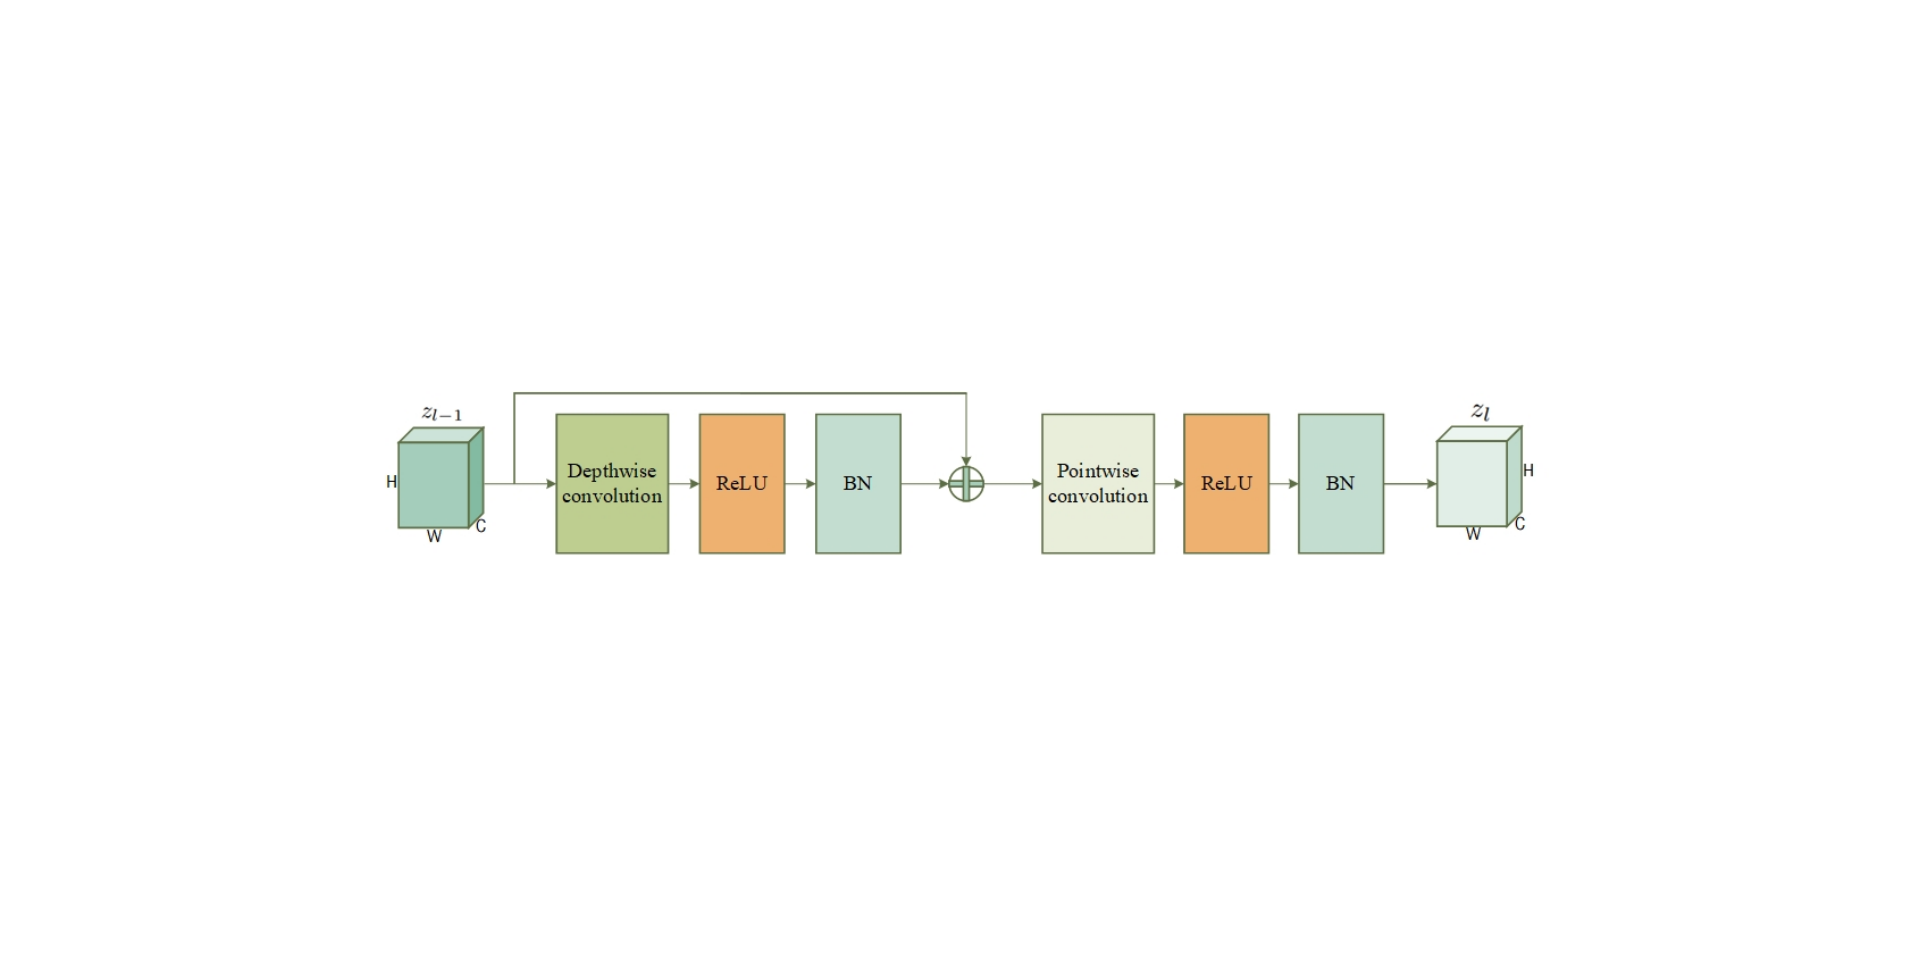
\includegraphics[width=\textwidth]{ConvMixer.png}
        \caption{ConvMixer}
        \label{fig:convmixer}
    \end{minipage}
    \hspace{0.5cm}
    \begin{minipage}[b]{0.5\linewidth}
        \centering
        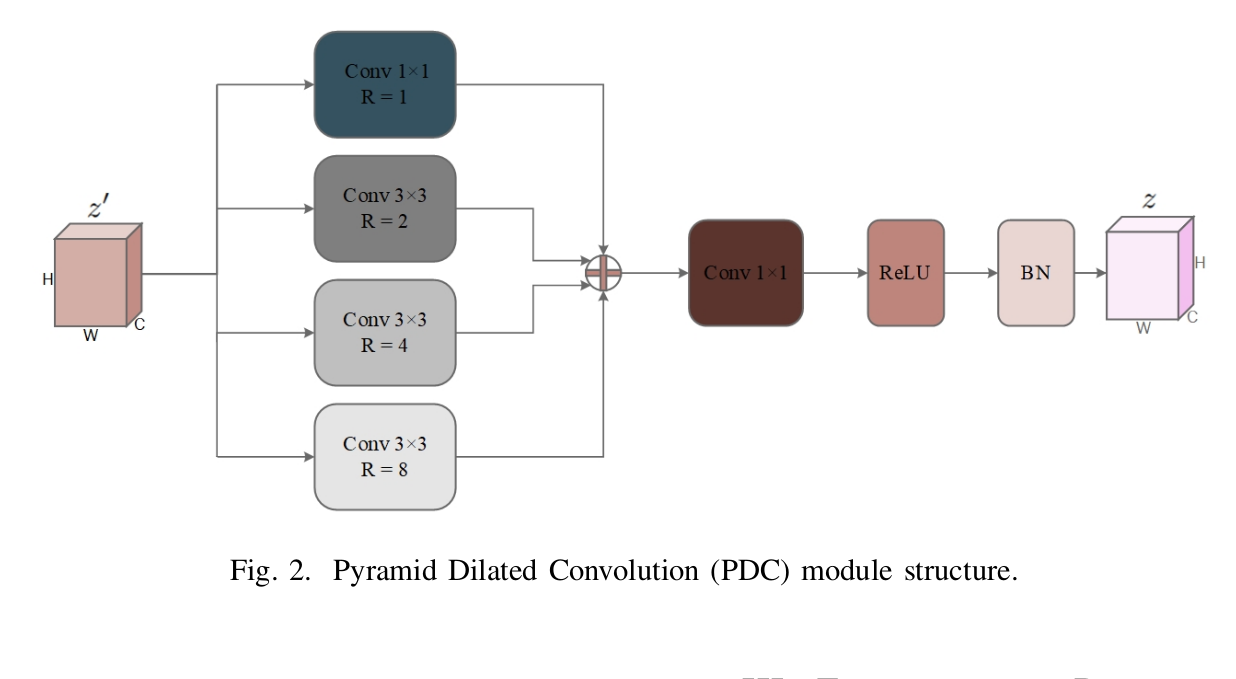
\includegraphics[width=\textwidth]{PDC.png}
        \caption{PDC Layer}
        \label{fig:pdc}
    \end{minipage}
    \end{figure}
\end{frame}

\begin{frame}{The CUNet}
    \begin{figure}[H]
        \centering
        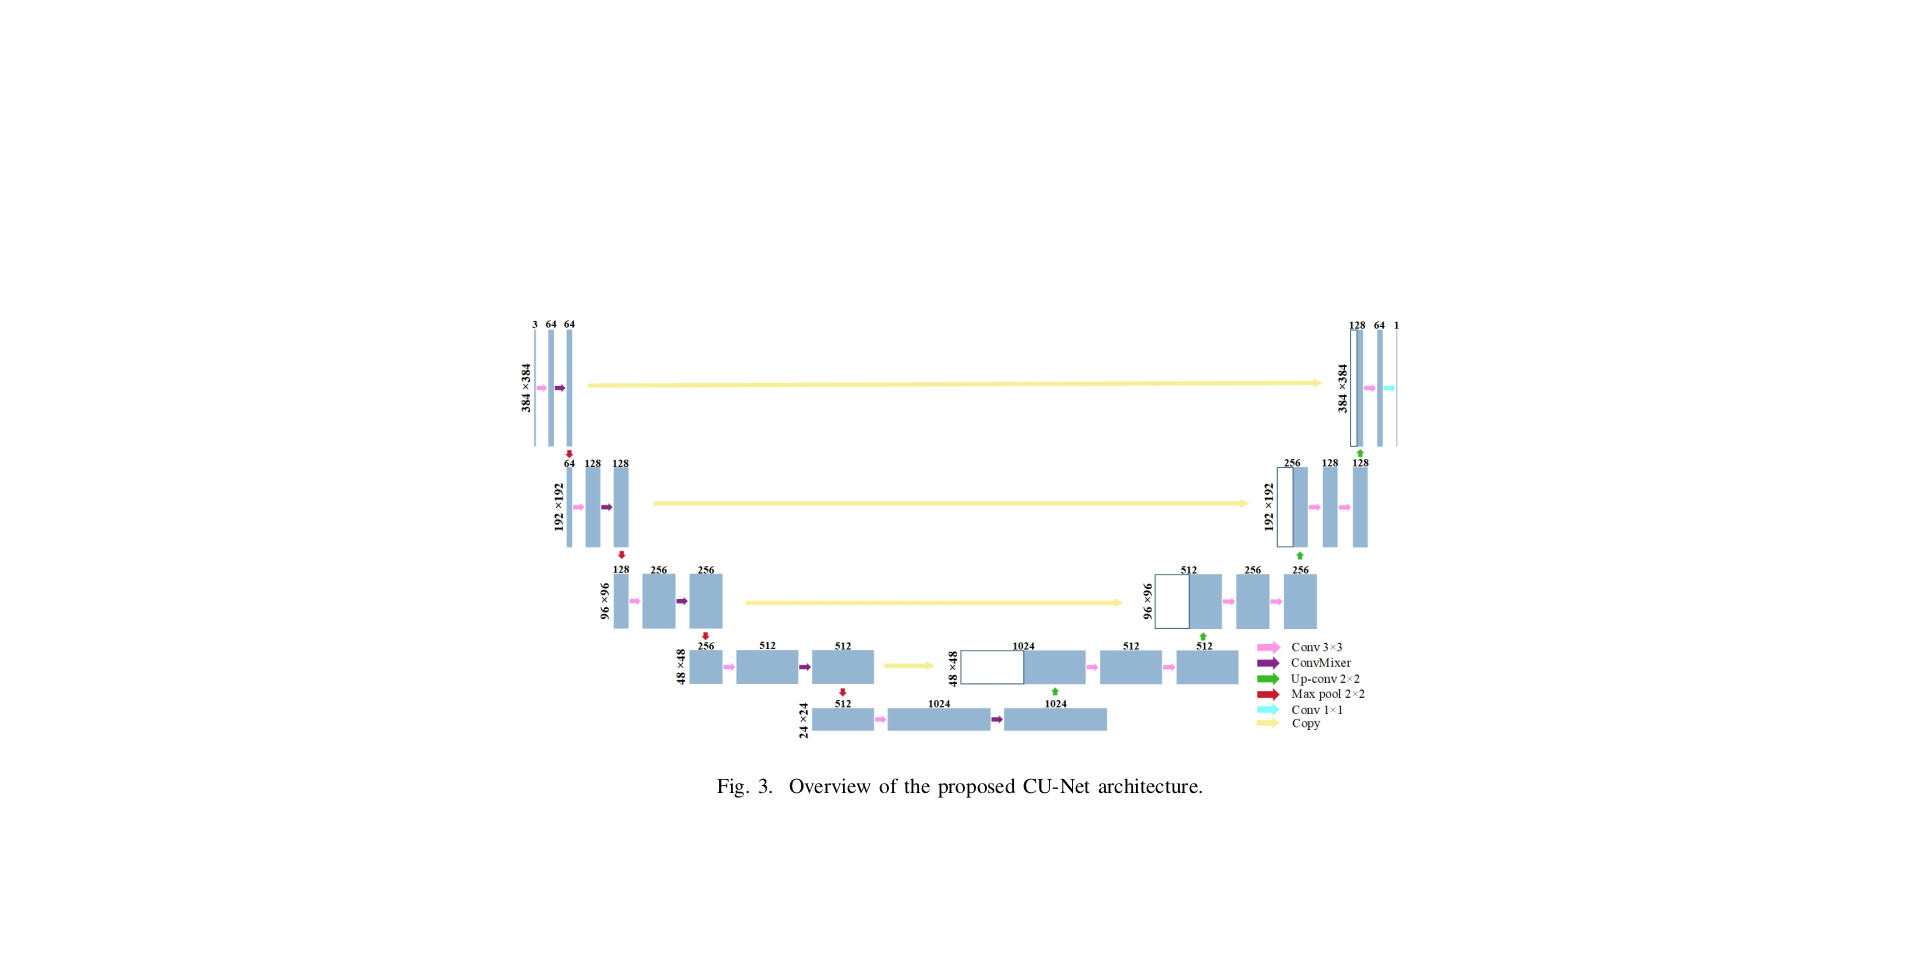
\includegraphics[width=\textwidth]{cunet.jpg}
        \caption{The CU-Net}
        \label{fig:b}
\end{figure}
\end{frame}
\begin{frame}{Architecture of UNet}
    \begin{enumerate}
        \item UNet consists of a contracting path (encoder) and an expansive path (decoder) with skip connections.
        \item In the encoder section, the goal is to receive the ultrasound image as input and achieve a condensed 
        representation of the input image.
        \item The decoder section decodes the information extracted from the encoder stage to the size of the input image.
        \item In U-Net, skip connections are direct connections between corresponding layers in the contracting
        path (encoder) and the expanding path (decoder), facilitating the seamless flow of high-resolution spatial 
        information to the decoding layers and aiding in the precise localization of features, thereby improving the 
        segmentation accuracy.
    \end{enumerate}
\end{frame}
\begin{frame}{Why PCUNet?}
    \begin{itemize}
        \item The CUNet differs from the UNet in that is has a ConvMixer block instead of the convolutional layer of the UNet for 
        each of the encoder blocks except the last one.
        \item The PCUNet has a PDC layer in the place of a ConvMixer block in the last encoder block.
        \item The ConvMixer module captures global context information by utilizing large-size kernels. The PDC module integrates local
        and global contextual patterns through utilization of parallel dilated convolution with different dilation rate. Furthermore,
        this model has fewer parameters than U-Net. We have replicated the results of the paper on the dataset Multi-Modality Ovarian Tumor Ultrasound
        (MMOTU)which includes two subsets with two modes, OUT 2d and OUT CEUS, containing 1469 2D ultrasound images and 
        170 CEUS images, respectively. We have worked on the OUT 2d subset.
    \end{itemize}
\end{frame}




\begin{frame}{Results : UNet}
    \begin{figure}[H]
        \centering
        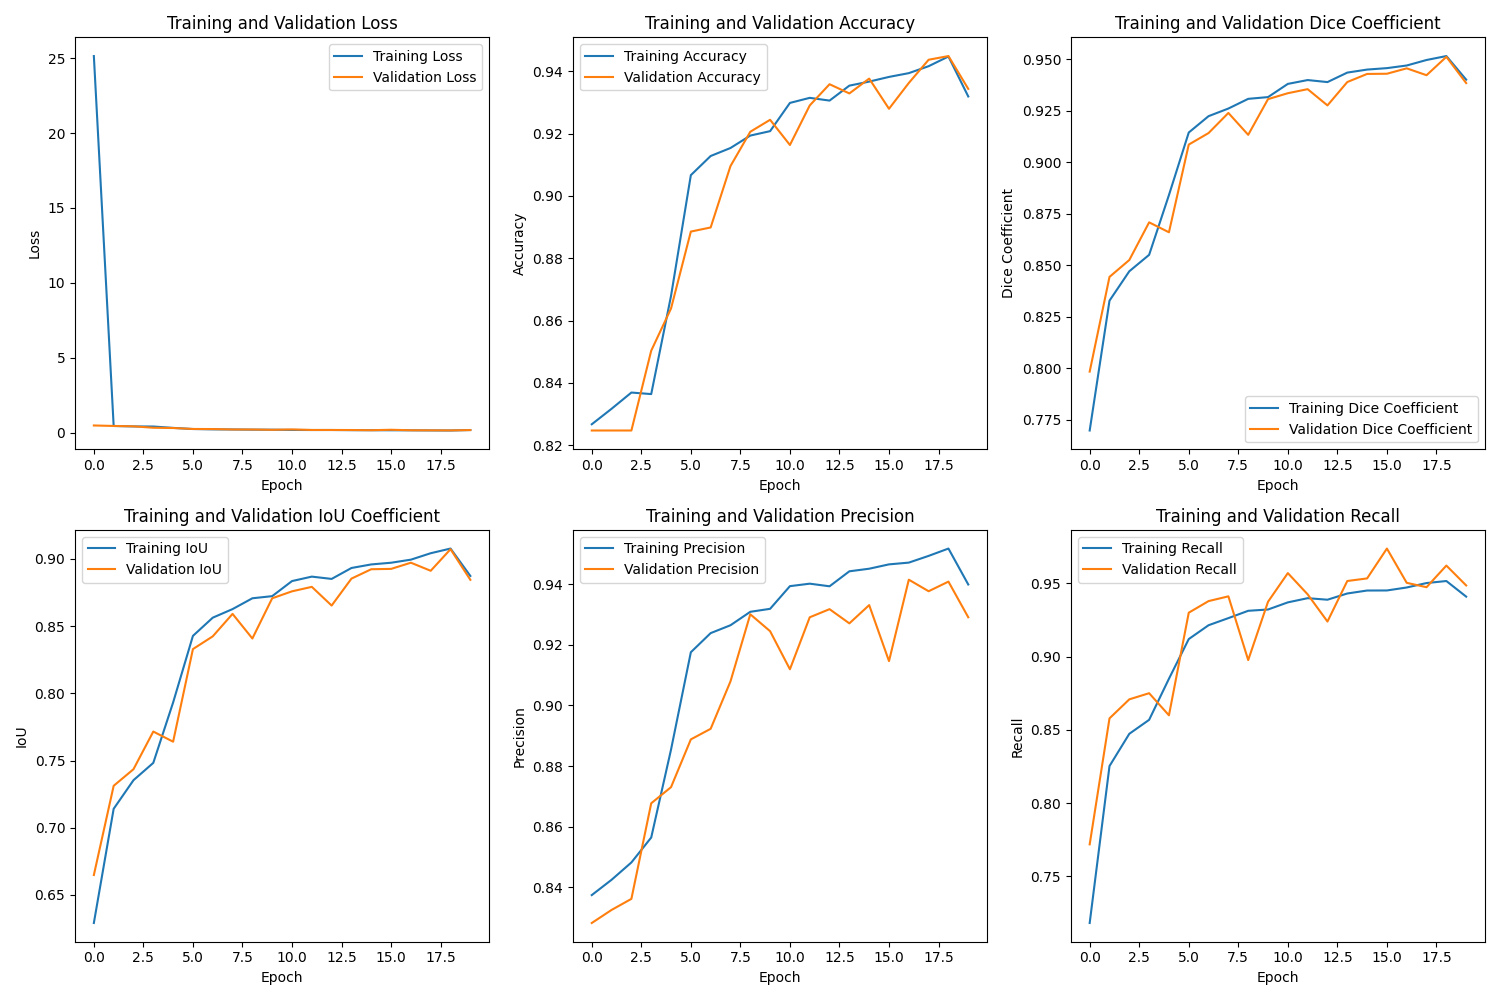
\includegraphics[width=\textwidth]{unet_metrics.png}
        \caption{Seeded Image}
        \label{fig:RU}
    \end{figure}
\end{frame}

\begin{frame}{Results : CUNet}
    \begin{figure}[H]
        \centering
        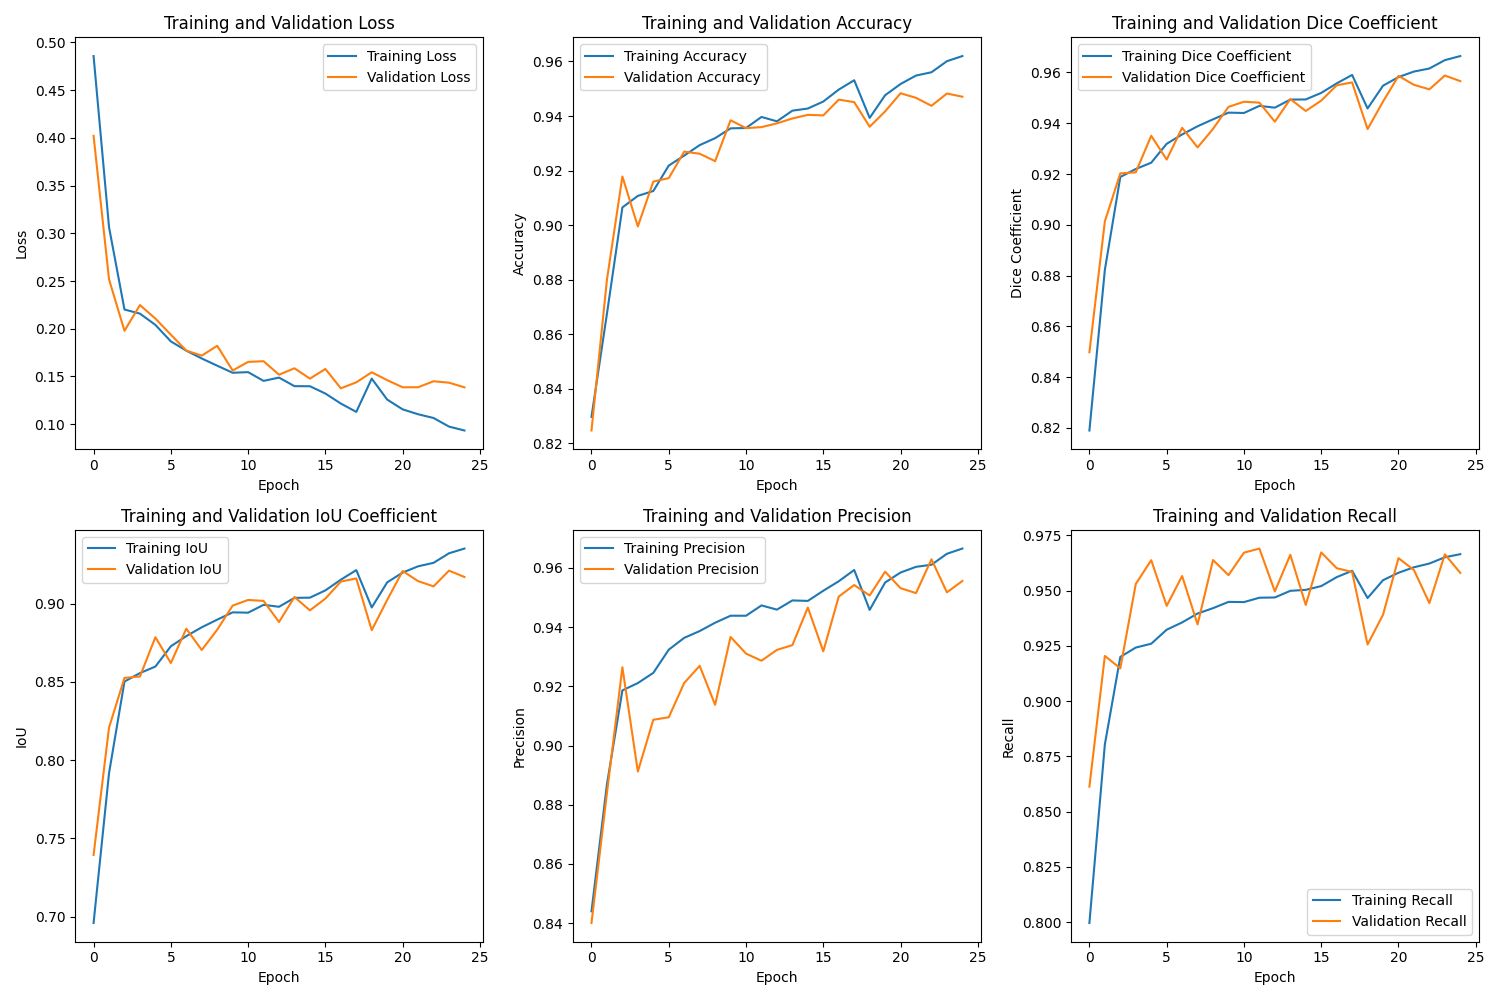
\includegraphics[width=\textwidth]{cunet_metrics.png}
        \caption{Seeded Image}
        \label{fig:RCU}
    \end{figure}
\end{frame}

\begin{frame}{Results : PCUNet}
    \begin{figure}[H]
            \centering
            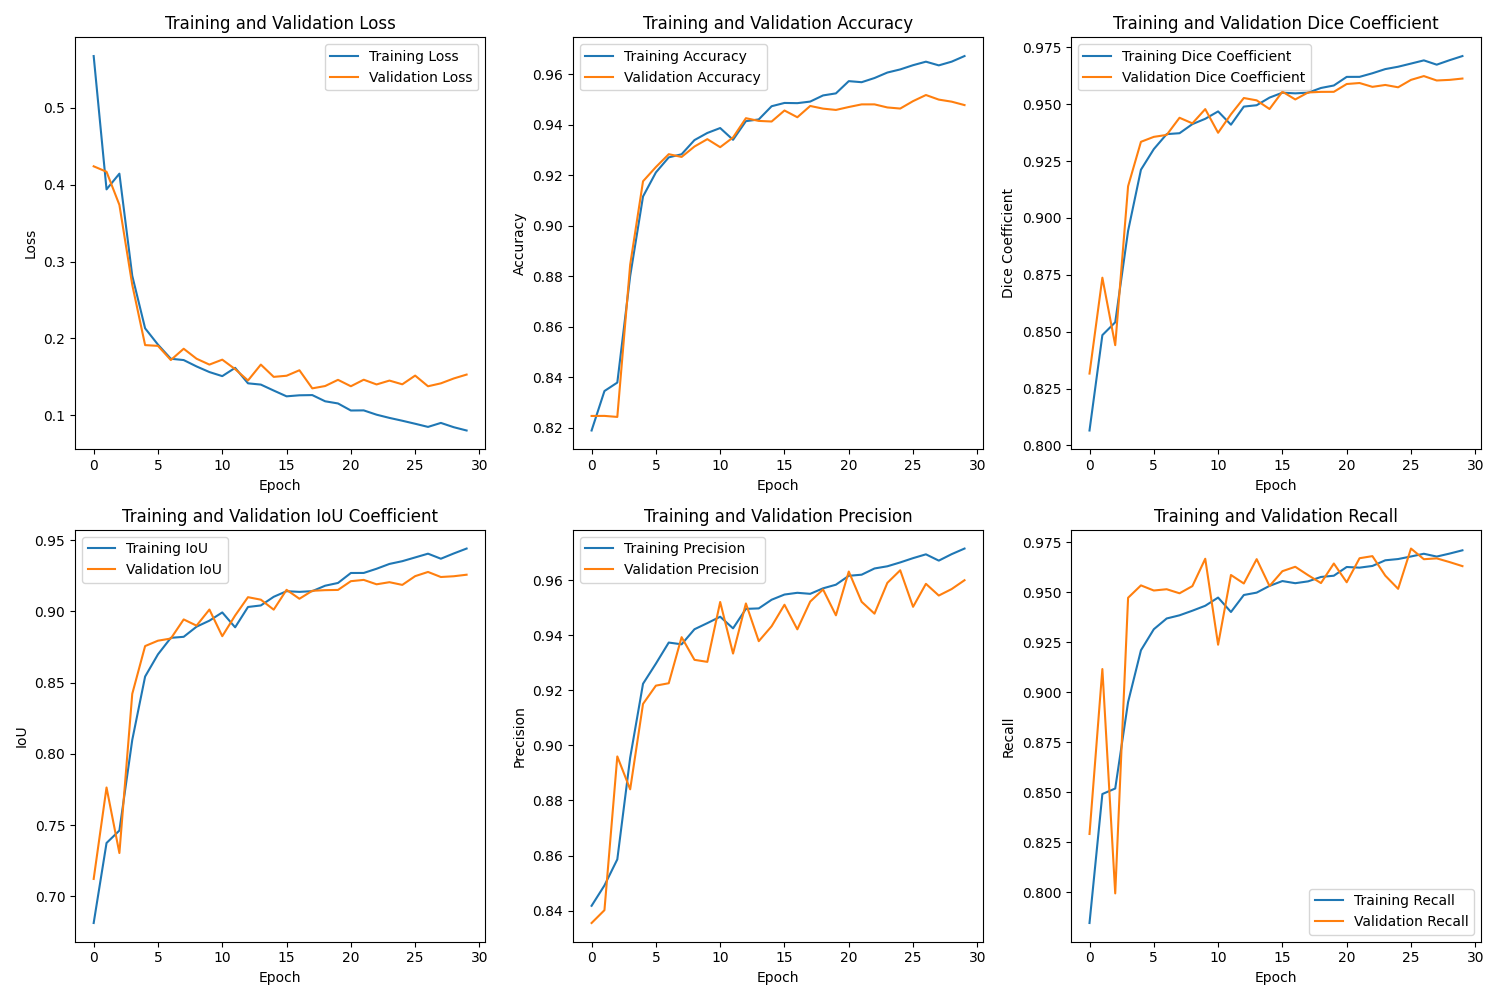
\includegraphics[width=\textwidth]{pcunet_metrics.png}
            \caption{Seeded Image}
            \label{fig:RPCU}
    \end{figure}
\end{frame}

\begin{frame}{Summary}
    \begin{table}[htbp]
        \centering
        \label{tab:performance}
        \begin{tabular}{|l|l|l|l|}
        \hline
        \textbf{Method} & \textbf{U-Net} & \textbf{CU-Net} & \textbf{PCU-Net} \\ \hline
        IoU              & $0.8868$ & $0.9352$ & $0.9440$ \\ \hline
        DSC              & $0.9399$ & $0.9665$ & $0.9712$ \\ \hline
        Precision        & $0.9401$ & $0.9666$ & $0.9715$ \\ \hline
        Recall           & $0.9399$ & $0.9665$ & $0.9710$ \\ \hline
        Accuracy         & $0.9319$ & $0.9620$ & $0.9673$ \\ \hline
        \end{tabular}
        \caption{Performance Comparison}

        \end{table}
        Clearly the PCUNet has better performance metrics than the CUNet and UNet models.
\end{frame}

% \begin{frame}{Improvements and Other Techniques}
% One improvement that can be made in the graph construction, is that instead of using infinite weight edges for seeded $t$-links, we could instead assign infinite weight edges for the seeded vertices, and use a Gaussian Mixture Model with respect to these vertices and assign edges from the source or sink to other vertices, proportional to the value using the GMM.\\
% \vspace{20pt}
% Another possible tweak in the model, is using directed graphs instead of undirected graphs. The directed link between vertices $p$ and $q$, in this case, can be assigned a weight $w_{p,q} = max(0,B_{p,q} - h(I_p - I_q))$. The value of $h$ can be tweaked in this case.\\
% \vspace{20pt}
% It is also possible to implement better algorithms to solve the max-flow min-cut problem.
% \end{frame}
\begin{frame}{References}
    \begin{enumerate}
        \item The paper https://ieeexplore.ieee.org/document/10491156
        \item Reference code https://towardsdatascience.com/cook-your-first-u-net-in-pytorch-b3297a844cf3
    \end{enumerate}
\end{frame}
\end{document}